% Options for packages loaded elsewhere
\PassOptionsToPackage{unicode}{hyperref}
\PassOptionsToPackage{hyphens}{url}
\PassOptionsToPackage{dvipsnames,svgnames,x11names}{xcolor}
%
\documentclass[
]{article}

\usepackage{amsmath,amssymb}
\usepackage{lmodern}
\usepackage{iftex}
\ifPDFTeX
  \usepackage[T1]{fontenc}
  \usepackage[utf8]{inputenc}
  \usepackage{textcomp} % provide euro and other symbols
\else % if luatex or xetex
  \usepackage{unicode-math}
  \defaultfontfeatures{Scale=MatchLowercase}
  \defaultfontfeatures[\rmfamily]{Ligatures=TeX,Scale=1}
\fi
% Use upquote if available, for straight quotes in verbatim environments
\IfFileExists{upquote.sty}{\usepackage{upquote}}{}
\IfFileExists{microtype.sty}{% use microtype if available
  \usepackage[]{microtype}
  \UseMicrotypeSet[protrusion]{basicmath} % disable protrusion for tt fonts
}{}
\makeatletter
\@ifundefined{KOMAClassName}{% if non-KOMA class
  \IfFileExists{parskip.sty}{%
    \usepackage{parskip}
  }{% else
    \setlength{\parindent}{0pt}
    \setlength{\parskip}{6pt plus 2pt minus 1pt}}
}{% if KOMA class
  \KOMAoptions{parskip=half}}
\makeatother
\usepackage{xcolor}
\usepackage[margin=3cm]{geometry}
\setlength{\emergencystretch}{3em} % prevent overfull lines
\setcounter{secnumdepth}{-\maxdimen} % remove section numbering
% Make \paragraph and \subparagraph free-standing
\ifx\paragraph\undefined\else
  \let\oldparagraph\paragraph
  \renewcommand{\paragraph}[1]{\oldparagraph{#1}\mbox{}}
\fi
\ifx\subparagraph\undefined\else
  \let\oldsubparagraph\subparagraph
  \renewcommand{\subparagraph}[1]{\oldsubparagraph{#1}\mbox{}}
\fi


\providecommand{\tightlist}{%
  \setlength{\itemsep}{0pt}\setlength{\parskip}{0pt}}\usepackage{longtable,booktabs,array}
\usepackage{calc} % for calculating minipage widths
% Correct order of tables after \paragraph or \subparagraph
\usepackage{etoolbox}
\makeatletter
\patchcmd\longtable{\par}{\if@noskipsec\mbox{}\fi\par}{}{}
\makeatother
% Allow footnotes in longtable head/foot
\IfFileExists{footnotehyper.sty}{\usepackage{footnotehyper}}{\usepackage{footnote}}
\makesavenoteenv{longtable}
\usepackage{graphicx}
\makeatletter
\def\maxwidth{\ifdim\Gin@nat@width>\linewidth\linewidth\else\Gin@nat@width\fi}
\def\maxheight{\ifdim\Gin@nat@height>\textheight\textheight\else\Gin@nat@height\fi}
\makeatother
% Scale images if necessary, so that they will not overflow the page
% margins by default, and it is still possible to overwrite the defaults
% using explicit options in \includegraphics[width, height, ...]{}
\setkeys{Gin}{width=\maxwidth,height=\maxheight,keepaspectratio}
% Set default figure placement to htbp
\makeatletter
\def\fps@figure{htbp}
\makeatother
\newlength{\cslhangindent}
\setlength{\cslhangindent}{1.5em}
\newlength{\csllabelwidth}
\setlength{\csllabelwidth}{3em}
\newlength{\cslentryspacingunit} % times entry-spacing
\setlength{\cslentryspacingunit}{\parskip}
\newenvironment{CSLReferences}[2] % #1 hanging-ident, #2 entry spacing
 {% don't indent paragraphs
  \setlength{\parindent}{0pt}
  % turn on hanging indent if param 1 is 1
  \ifodd #1
  \let\oldpar\par
  \def\par{\hangindent=\cslhangindent\oldpar}
  \fi
  % set entry spacing
  \setlength{\parskip}{#2\cslentryspacingunit}
 }%
 {}
\usepackage{calc}
\newcommand{\CSLBlock}[1]{#1\hfill\break}
\newcommand{\CSLLeftMargin}[1]{\parbox[t]{\csllabelwidth}{#1}}
\newcommand{\CSLRightInline}[1]{\parbox[t]{\linewidth - \csllabelwidth}{#1}\break}
\newcommand{\CSLIndent}[1]{\hspace{\cslhangindent}#1}

\makeatletter
\makeatother
\makeatletter
\makeatother
\makeatletter
\@ifpackageloaded{caption}{}{\usepackage{caption}}
\AtBeginDocument{%
\ifdefined\contentsname
  \renewcommand*\contentsname{Table of contents}
\else
  \newcommand\contentsname{Table of contents}
\fi
\ifdefined\listfigurename
  \renewcommand*\listfigurename{List of Figures}
\else
  \newcommand\listfigurename{List of Figures}
\fi
\ifdefined\listtablename
  \renewcommand*\listtablename{List of Tables}
\else
  \newcommand\listtablename{List of Tables}
\fi
\ifdefined\figurename
  \renewcommand*\figurename{Figure}
\else
  \newcommand\figurename{Figure}
\fi
\ifdefined\tablename
  \renewcommand*\tablename{Table}
\else
  \newcommand\tablename{Table}
\fi
}
\@ifpackageloaded{float}{}{\usepackage{float}}
\floatstyle{ruled}
\@ifundefined{c@chapter}{\newfloat{codelisting}{h}{lop}}{\newfloat{codelisting}{h}{lop}[chapter]}
\floatname{codelisting}{Listing}
\newcommand*\listoflistings{\listof{codelisting}{List of Listings}}
\makeatother
\makeatletter
\@ifpackageloaded{caption}{}{\usepackage{caption}}
\@ifpackageloaded{subcaption}{}{\usepackage{subcaption}}
\makeatother
\makeatletter
\@ifpackageloaded{tcolorbox}{}{\usepackage[many]{tcolorbox}}
\makeatother
\makeatletter
\@ifundefined{shadecolor}{\definecolor{shadecolor}{rgb}{.97, .97, .97}}
\makeatother
\makeatletter
\makeatother
\ifLuaTeX
  \usepackage{selnolig}  % disable illegal ligatures
\fi
\IfFileExists{bookmark.sty}{\usepackage{bookmark}}{\usepackage{hyperref}}
\IfFileExists{xurl.sty}{\usepackage{xurl}}{} % add URL line breaks if available
\urlstyle{same} % disable monospaced font for URLs
\hypersetup{
  pdftitle={Optimization of real state investment portfolio using R},
  pdfauthor={Ariel Levy\^{}\{1\}; Marcus Antonio Cardoso Ramalho\^{}\{1\}},
  pdfkeywords={real state investment; portfolio optmization; Fundos de
investimento imobiliário; Sharpe ratio; portfolio risk},
  colorlinks=true,
  linkcolor={blue},
  filecolor={Maroon},
  citecolor={Blue},
  urlcolor={Blue},
  pdfcreator={LaTeX via pandoc}}

\title{Optimization of real state investment portfolio using R}
\author{Ariel Levy\(^{1}\); Marcus Antonio Cardoso Ramalho\(^{1}\)}
\date{}

\begin{document}
\begin{flushright}

\includegraphics[angle=0,keepaspectratio,width=3cm]{logo.pdf}
\end{flushright}

\noindent {\small \textsl{IX Xornada de Usuarios de R en Galicia\textsl{\ \newline Santiago de Compostela}, 20 de outubro do 2022}} \vspace{20pt}

\begin{center}
\textbf{Optimization of real state investment portfolio using R}

\vspace{0.15cm}

Ariel Levy\(^{1}\); Marcus Antonio Cardoso Ramalho\(^{1}\) 
\end{center}

\vspace{0.06cm}

$^{1}$ 
Universidade Federal Fluminense - PPGAD
\begin{center}
\textbf{ABSTRACT}
\end{center}

\begin{quotation}
\noindent This resume discuss a method of real state funds investment
portifolio optmization using R with the packages tidyverse and quantmod
\end{quotation}

\vspace{0.4cm}

\textbf{Keywords}:real state investment; portfolio optmization; Fundos
de investimento imobiliário; Sharpe ratio; portfolio risk

\vspace{0.4cm}

\ifdefined\Shaded\renewenvironment{Shaded}{\begin{tcolorbox}[frame hidden, interior hidden, enhanced, boxrule=0pt, borderline west={3pt}{0pt}{shadecolor}, sharp corners, breakable]}{\end{tcolorbox}}\fi

\pagestyle{empty}
\setlength\parindent{0pt}

\begin{center}
\textbf{1. INTRODUCTION}
\end{center}

This work is part of Marcus Ramalho undeargraduation final project in
administration on Universidade Federal Fluminense and advised by Ariel
Levy, entitled: Análise de risco e rentabilidade de uma carteira de
fundos de investimento imobiliário.

The project addresses the data acquisition for optimizing Real Estate
Investment Funds{[}1{]}, FIIs. The code was adapted from several sources
and built in, using the knowledge acquired by the student during the
first covid-19 pandemic year when Ariel Levy offered a remote course on
finance with R for administration students.

To better understand this project, first, we need to present some simple
concepts about FII and risk in finance. First, FII or Fundo de
Investimento Imobiliário is a booming type of real estate investment in
Brazil. There were more than one million investors in 2020, their small
majority investor, compared with 2010 when there were less than fifty
thousand investors. The market's growth is notable. The appeal of this
investment is related to the changes in the Brazilian economy after
2016. With the lowest basic interest rate ever, market players saw in
FII an opportunity to beat risk-free investments (figure 1), with a
lower risk than other equity assets.

\begin{figure}

{\centering 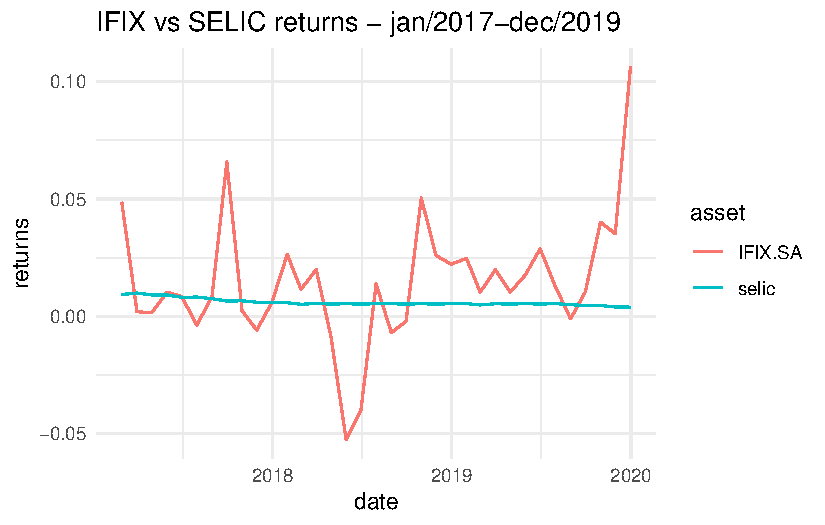
\includegraphics{FII_portfolio_opt_R_files/figure-pdf/Graph_1-1.pdf}

}

\caption{returns compared - ggplot2}

\end{figure}

\begin{center}
\textbf{2. OBJECTIVE}
\end{center}

This project aimed to simulate an optimized FII portfolio considering
the scenario of a low Brazilian risk-free interest rate and an
accelerated real state market growth, focusing on some market indicators
such as:

The covariance and the standard deviation to measure volatility and
risk.

Sharpe ratio{[}2{]}, which measures the adjusted profitability (\(P_r\))
for the total portfolio risk (\(\sigma\)), compared with a minimum
accepted return (\(M_r\)).

\[ SI=\frac{\overline{P_r}-M_r}{\sigma_{p}} \]

Capital asset pricing model(CAPM){[}3{]}, \(\beta\), witch, measures the
portfolio risk sensibility to a specified non-diversifiable risk asset ,
here the IFIX was used as
reference.\[\beta=\frac{Cov(P;IFIX)}{\sigma_{IFIX}^2}\]

\begin{center}
\textbf{3. METODOLOGY}
\end{center}

This work relied on the use of RStudio and various R packages to
manipulate and understand the data, including Tydiverse {[}4{]},
Lubridade{[}5{]}for general data manipulation, plotly{[}6{]}, and
ggplot2{[}7{]} for data visualization and quantmode{[}8{]},
tidyquant{[}9{]} and PerformanceAnalitycs{[}10{]} for financial data
vesting, manipulation, and computation.

For the asset selection, some assumptions were made, like a filter tool
from the website Clube do FII{[}1{]} to select all assets with the IPO
(Inicial public offering) before 2017 and mean monthly liquidity greater
than R\$ 2,000.00. The chosen asset price data was downloaded within the
time window from 2017 to 2019 with the package quantmod{[}8{]}and Yahoo
Finance{[}11{]} as a source. After the price data vesting, follow the
monthly log returns calculation using dplyr{[}12{]} and xts{[}13{]} to
transform the daily returns into monthly returns. Moreover, discarding
all funds with inconsistent data or participation in the market index
(IFIX) resulted in 24 assets selected.

Before we begin the simulations and optimization with the selected
portfolio, we set a weight vector with a value for each asset. And the
optimization took part by adapting a script from
codingfinance.com{[}14{]} and calculating the portfolio returns using
weights generated with the base function runif{[}15{]}, which uses
uniform distribution. Finally, the market indicators were computed and
filtered to show the tangent and minimum variance.

\begin{center}
\textbf{3. DISCUSSION AND CONCLUSION}
\end{center}

\hypertarget{references}{%
\subsection*{References}\label{references}}
\addcontentsline{toc}{subsection}{References}

\hypertarget{refs}{}
\begin{CSLReferences}{0}{0}
\leavevmode\vadjust pre{\hypertarget{ref-clubefii2020}{}}%
\CSLLeftMargin{{[}1{]} }%
\CSLRightInline{ClubeFII. \href{https://www.clubefii.com.br}{Clube FII -
O maior site de Fundos Imobiliários do Brasil} 2020.}

\leavevmode\vadjust pre{\hypertarget{ref-sharpe1994}{}}%
\CSLLeftMargin{{[}2{]} }%
\CSLRightInline{Sharpe WF. The Sharpe Ratio. The Journal of Portfolio
Management 1994;21:49--58.
\url{https://doi.org/10.3905/jpm.1994.409501}.}

\leavevmode\vadjust pre{\hypertarget{ref-sharpe1964}{}}%
\CSLLeftMargin{{[}3{]} }%
\CSLRightInline{Sharpe WF. CAPITAL ASSET PRICES: A THEORY OF MARKET
EQUILIBRIUM UNDER CONDITIONS OF RISK*. The Journal of Finance
1964;19:425--42.
\url{https://doi.org/10.1111/j.1540-6261.1964.tb02865.x}.}

\leavevmode\vadjust pre{\hypertarget{ref-wickhamWelcomeTidyverse2019a}{}}%
\CSLLeftMargin{{[}4{]} }%
\CSLRightInline{Wickham H, Averick M, Bryan J, Chang W, McGowan L,
François R, et al. Welcome to the {Tidyverse}. Journal of Open Source
Software 2019;4:1686. \url{https://doi.org/10.21105/joss.01686}.}

\leavevmode\vadjust pre{\hypertarget{ref-grolemundDatesTimesMade2011}{}}%
\CSLLeftMargin{{[}5{]} }%
\CSLRightInline{Grolemund G, Wickham H. Dates and {Times} {Made} {Easy}
with \textbf{lubridate}. Journal of Statistical Software 2011;40.
\url{https://doi.org/10.18637/jss.v040.i03}.}

\leavevmode\vadjust pre{\hypertarget{ref-sievertInteractiveWebbasedData2022}{}}%
\CSLLeftMargin{{[}6{]} }%
\CSLRightInline{Sievert C. \href{https://plotly-r.com/}{Interactive
web-based data visualization with {R}, plotly, and shiny}. 2022.}

\leavevmode\vadjust pre{\hypertarget{ref-wickham2016}{}}%
\CSLLeftMargin{{[}7{]} }%
\CSLRightInline{Wickham H. ggplot2: Elegant graphics for data analysis.
New York, NY: Springer Science+Business Media, LLC; 2016.}

\leavevmode\vadjust pre{\hypertarget{ref-ryanQuantmodQuantitativeFinancial2022}{}}%
\CSLLeftMargin{{[}8{]} }%
\CSLRightInline{Ryan JA, Ulrich JM, Smith EB, Thielen W, Teetor P,
Bronder S. \href{https://CRAN.R-project.org/package=quantmod}{Quantmod:
{Quantitative} {Financial} {Modelling} {Framework}} 2022.}

\leavevmode\vadjust pre{\hypertarget{ref-danchoTidyquantTidyQuantitative2022}{}}%
\CSLLeftMargin{{[}9{]} }%
\CSLRightInline{Dancho M, Vaughan D.
\href{https://CRAN.R-project.org/package=tidyquant}{Tidyquant: {Tidy}
{Quantitative} {Financial} {Analysis}} 2022.}

\leavevmode\vadjust pre{\hypertarget{ref-petersonPerformanceAnalyticsEconometricTools2020}{}}%
\CSLLeftMargin{{[}10{]} }%
\CSLRightInline{Peterson BG, Carl P, Boudt K, Bennett R, Ulrich J, Zivot
E, et al.
\href{https://CRAN.R-project.org/package=PerformanceAnalytics}{{PerformanceAnalytics}:
{Econometric} {Tools} for {Performance} and {Risk} {Analysis}} 2020.}

\leavevmode\vadjust pre{\hypertarget{ref-YahooFinance2022}{}}%
\CSLLeftMargin{{[}11{]} }%
\CSLRightInline{\href{https://finance.yahoo.com/}{Yahoo {Finance}}
2022.}

\leavevmode\vadjust pre{\hypertarget{ref-wickhamDplyrGrammarData2022}{}}%
\CSLLeftMargin{{[}12{]} }%
\CSLRightInline{Wickham H, François R, Henry L, Müller K, RStudio.
\href{https://CRAN.R-project.org/package=dplyr}{Dplyr: {A} {Grammar} of
{Data} {Manipulation}} 2022.}

\leavevmode\vadjust pre{\hypertarget{ref-ryanXtsEXtensibleTime2020}{}}%
\CSLLeftMargin{{[}13{]} }%
\CSLRightInline{Ryan JA, Ulrich JM, Bennett R, Joy C.
\href{https://CRAN.R-project.org/package=xts}{Xts: {eXtensible} {Time}
{Series}} 2020.}

\leavevmode\vadjust pre{\hypertarget{ref-CodingFinance0000}{}}%
\CSLLeftMargin{{[}14{]} }%
\CSLRightInline{\href{https://www.codingfinance.com/post/2018-05-31-portfolio-opt-in-r/}{Coding
{Finance}}. Portfolio Optimization in R.}

\leavevmode\vadjust pre{\hypertarget{ref-rcoreteamLanguageEnvironmentStatistical2022}{}}%
\CSLLeftMargin{{[}15{]} }%
\CSLRightInline{Team RC. \href{https://www.r-project.org/}{R: {A}
{Language} and {Environment} for {Statistical} {Computing}} 2022.}

\end{CSLReferences}



\end{document}
